\begin{equation}
    \begin{aligned}
        \begin{gathered}
            \begin{tikzpicture}[x=0.75pt,y=0.75pt,yscale=-0.7,xscale=0.7]
                %uncomment if require: \path (0,300); %set diagram left start at 0, and has height of 300
                
                %Straight Lines [id:da9158108405032224] 
                \draw  [dash pattern={on 4.5pt off 4.5pt}]  (226.71,140) -- (290,140)(226.71,143) -- (290,143) ;
                \end{tikzpicture}
        \end{gathered} \quad &= \quad \begin{gathered}
            \begin{tikzpicture}[x=0.75pt,y=0.75pt,yscale=-0.7,xscale=0.7]
                %uncomment if require: \path (0,300); %set diagram left start at 0, and has height of 300
                
                %Straight Lines [id:da9158108405032224] 
                \draw  [dash pattern={on 4.5pt off 4.5pt}]  (213.71,159) -- (290,159) ;
            \end{tikzpicture} 
        \end{gathered} \quad + \quad \begin{gathered}
            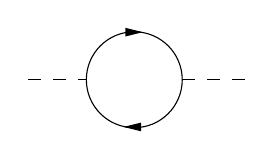
\begin{tikzpicture}[x=0.75pt,y=0.75pt,yscale=-0.7,xscale=0.7]
                %uncomment if require: \path (0,300); %set diagram left start at 0, and has height of 300
                
                %Straight Lines [id:da0014168747947034266] 
                \draw  [dash pattern={on 4.5pt off 4.5pt}]  (140.71,142) -- (180.71,142) ;
                %Shape: Circle [id:dp6136073910163897] 
                \draw   (180.71,142) .. controls (180.71,123.77) and (195.48,109) .. (213.71,109) .. controls (231.93,109) and (246.71,123.77) .. (246.71,142) .. controls (246.71,160.23) and (231.93,175) .. (213.71,175) .. controls (195.48,175) and (180.71,160.23) .. (180.71,142) -- cycle ;
                %Straight Lines [id:da24276323775928632] 
                \draw    (219.5,109.25) ;
                \draw [shift={(219.5,109.25)}, rotate = 180] [fill={rgb, 255:red, 0; green, 0; blue, 0 }  ][line width=0.08]  [draw opacity=0] (12,-3) -- (0,0) -- (12,3) -- cycle    ;
                %Straight Lines [id:da5824966682961659] 
                \draw    (212.33,174.5) -- (208.33,174.5) ;
                \draw [shift={(206.33,174.5)}, rotate = 360] [fill={rgb, 255:red, 0; green, 0; blue, 0 }  ][line width=0.08]  [draw opacity=0] (12,-3) -- (0,0) -- (12,3) -- cycle    ;
                %Straight Lines [id:da5514620719913015] 
                \draw  [dash pattern={on 4.5pt off 4.5pt}]  (246.71,142) -- (292,142) ;
                \end{tikzpicture}                
        \end{gathered} \quad + \cdots  \\
        & \quad \quad + \quad \begin{gathered}
            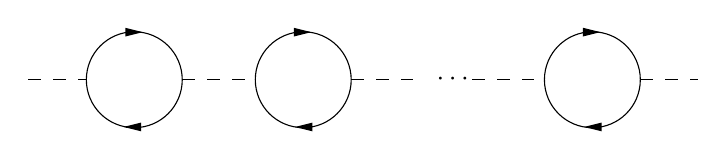
\begin{tikzpicture}[x=0.75pt,y=0.75pt,yscale=-0.7,xscale=0.7]
                %uncomment if require: \path (0,300); %set diagram left start at 0, and has height of 300
                
                %Straight Lines [id:da3963818408569353] 
                \draw  [dash pattern={on 4.5pt off 4.5pt}]  (100.71,140) -- (140.71,140) ;
                %Shape: Circle [id:dp49286917160300825] 
                \draw   (140.71,140) .. controls (140.71,121.77) and (155.48,107) .. (173.71,107) .. controls (191.93,107) and (206.71,121.77) .. (206.71,140) .. controls (206.71,158.23) and (191.93,173) .. (173.71,173) .. controls (155.48,173) and (140.71,158.23) .. (140.71,140) -- cycle ;
                %Straight Lines [id:da12799067746596915] 
                \draw    (179.5,107.25) ;
                \draw [shift={(179.5,107.25)}, rotate = 180] [fill={rgb, 255:red, 0; green, 0; blue, 0 }  ][line width=0.08]  [draw opacity=0] (12,-3) -- (0,0) -- (12,3) -- cycle    ;
                %Straight Lines [id:da840312664371196] 
                \draw    (172.33,172.5) -- (168.33,172.5) ;
                \draw [shift={(166.33,172.5)}, rotate = 360] [fill={rgb, 255:red, 0; green, 0; blue, 0 }  ][line width=0.08]  [draw opacity=0] (12,-3) -- (0,0) -- (12,3) -- cycle    ;
                %Straight Lines [id:da7934152347348731] 
                \draw  [dash pattern={on 4.5pt off 4.5pt}]  (206.71,140) -- (257,140) ;
                %Shape: Circle [id:dp8590618643032912] 
                \draw   (257,140) .. controls (257,121.77) and (271.77,107) .. (290,107) .. controls (308.23,107) and (323,121.77) .. (323,140) .. controls (323,158.23) and (308.23,173) .. (290,173) .. controls (271.77,173) and (257,158.23) .. (257,140) -- cycle ;
                %Straight Lines [id:da45688158211198093] 
                \draw    (295.5,107.25) ;
                \draw [shift={(295.5,107.25)}, rotate = 180] [fill={rgb, 255:red, 0; green, 0; blue, 0 }  ][line width=0.08]  [draw opacity=0] (12,-3) -- (0,0) -- (12,3) -- cycle    ;
                %Straight Lines [id:da45633743508297653] 
                \draw    (290.33,172.5) -- (286.33,172.5) ;
                \draw [shift={(284.33,172.5)}, rotate = 360] [fill={rgb, 255:red, 0; green, 0; blue, 0 }  ][line width=0.08]  [draw opacity=0] (12,-3) -- (0,0) -- (12,3) -- cycle    ;
                %Straight Lines [id:da3751639063231236] 
                \draw  [dash pattern={on 4.5pt off 4.5pt}]  (323,140) -- (373.29,140) ;
                %Straight Lines [id:da1040340540636353] 
                \draw  [dash pattern={on 4.5pt off 4.5pt}]  (406.29,140) -- (456.59,140) ;
                %Shape: Circle [id:dp20071411307184106] 
                \draw   (456,140) .. controls (456,121.77) and (470.77,107) .. (489,107) .. controls (507.23,107) and (522,121.77) .. (522,140) .. controls (522,158.23) and (507.23,173) .. (489,173) .. controls (470.77,173) and (456,158.23) .. (456,140) -- cycle ;
                %Straight Lines [id:da20812325261772835] 
                \draw    (494.5,107.25) ;
                \draw [shift={(494.5,107.25)}, rotate = 180] [fill={rgb, 255:red, 0; green, 0; blue, 0 }  ][line width=0.08]  [draw opacity=0] (12,-3) -- (0,0) -- (12,3) -- cycle    ;
                %Straight Lines [id:da8266206782881969] 
                \draw    (489.33,172.5) -- (485.33,172.5) ;
                \draw [shift={(483.33,172.5)}, rotate = 360] [fill={rgb, 255:red, 0; green, 0; blue, 0 }  ][line width=0.08]  [draw opacity=0] (12,-3) -- (0,0) -- (12,3) -- cycle    ;
                %Straight Lines [id:da7168426085353536] 
                \draw  [dash pattern={on 4.5pt off 4.5pt}]  (522,140) -- (562,140) ;
                
                % Text Node
                \draw (380,140) node [anchor=west] [inner sep=0.75pt]    {$\cdots $};
                \end{tikzpicture}            
        \end{gathered} \quad + \cdots .
    \end{aligned}
    \label{eq:rpa-diagram}
\end{equation}